\section{Architectural and design patterns}

\subsection{Architectural patterns}
Our software will be built around two main architectural patterns: \textit{Client-server}\ref{fig:androidclient-server} and \textit{Model-View-Controller} (MVC).

The MVC-pattern will be implemented together with client-server as follows: The model contains game instances, each of which contains two players and two game boards where each board contains ships. The view presents the game screen which consists of both game boards, a button select the active (larger) view, and a button to bomb a selected coordinates. The view allows the user to choose which coordinate to bomb using the screen's touch input and by confirming the choice with a button. When a bombing is confirmed, the controller on the server is notified through an HTTP request and takes the appropriate action. This pattern allows us to cleanly separate the user input and graphical representation from the business logic. You can see the relationship in figure \ref{fig:mvc+client-server}.

TThe models and controllers, which together make up the game logic, will be implemented server-side, while the client will implement the view. The clients and the server communicateso that user events in the view are reported to the controller, and the controller updates the
views’ contents as necessary. In actuality, the client will poll the server for changes, but logically the controller updates the view. 
\begin{figure}[h]
  \centering
    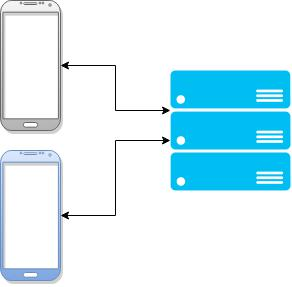
\includegraphics[width=60mm]{figs/androidclient-server.jpg}
  \caption{A figure describing the client-server architecture, with two Android clients.}
\label{fig:androidclient-server}
\end{figure}

\begin{figure}[h]
  \centering
    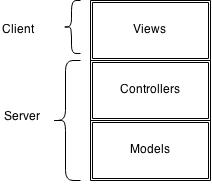
\includegraphics[width=60mm]{figs/mvc+client-server.jpg}
  \caption{A figure describing how the MVC architectural pattern will work witn the client-server architectura in our planned architecture.}
\label{fig:mvc+client-server}
\end{figure}


\subsection{Design patterns}
We will in addition to the above mentioned architectural patterns, we also plan to make use of the following design patterns:
% todo
\begin{description}
    \item{State-pattern} Both views on the client and game-object on the server will have states. 
    \item{Template-pattern} With the libgdx-library we'll have to extend the abstract Game- and Screen-classes to get a working Android application.
    \item{Observer-pattern} Buttons and other graphical elements will make use of this pattern to react on events from the user.
\end{description}